\section{Доп. Материалы}
\subsection{Микробенчмаркинг}

\begin{frame}[fragile]{Функции, спасающие от слишком умного компилятора}
	\begin{enumerate}
		\item Помогает сохранить какой-то объект, не дать компилятору в ходе оптимизации избавиться от объекта:
\begin{lstlisting}
    static void escape(void *p) {
        asm volatile ("" : : "g"(p) : "memory");
    }
\end{lstlisting}

		\item Похожая функция, указывающая, что в момент исполнения возможна запись в любую область памяти, что помогает не дать компилятору избавиться от \enquote{бесполезных} операторов:
\begin{lstlisting}
    static void clobber() {
        asm volatile ("" : : : "memory");
    }
\end{lstlisting}

	\end{enumerate}
\end{frame}

\begin{frame}[fragile]{Пример кода теста example.cpp}
	\tiny
\begin{lstlisting}
#include "benchmark.h"
#include <vector>

static void escape(void *p) { asm volatile ("" : : "g"(p) : "memory"); }
static void clobber() { asm volatile ("" : : : "memory"); }

static void bm_create(benchmark::State &state) {
   while (state.KeepRunning()) {
      std::vector<int> v;
      escape(&v);   
      (void) v;   } } BENCHMARK(bm_create);

static void bm_reserve(benchmark::State &state) {
   while (state.KeepRunning()) {
      std::vector<int> v;
      v.reserve(1);
      escape(v.data());   } } BENCHMARK(bm_reserve);

static void bm_push_back(benchmark::State &state) {
   while (state.KeepRunning()) {
      std::vector<int> v;
      escape(v.data());
      v.push_back(42);
      clobber();   } } BENCHMARK(bm_push_back);

BENCHMARK_MAIN();
\end{lstlisting}
\end{frame}

\begin{frame}[fragile]{Как скомпилировать для Google Benchmark правильно?}
	\begin{itemize}
		\item -O2 или -O3 флаг, ибо в реальности ваше приложение будет компилироваться с применением оптимизаций, а значит тестировать надо уже с ними (и с ними же бороться).
		\item -fno-omit-frame-pointer -- позволяет сохранять границы кадров стека, что требуется для адекватного отображения результата профилирования в perf report
	\end{itemize}
	Итоговый минимальный makefile:
	\tiny
\begin{lstlisting}
   example: example.cpp
       g++ example.cpp -L. -lbenchmark -lpthread -O3 -fno-omit-frame-pointer -o example
\end{lstlisting}

	\normalsize
	На всякий случай: в системе должна быть установлена, либо находиться рядом библиотека pthread, собственно библиотека benchmark.a, а так же ее заголовочный файл benchmark.h.
\end{frame}

\begin{frame}[fragile]{Запуск теста и просмотр результата}
	\begin{enumerate}
		\item Используем perf record для записи результата:
\begin{lstlisting}
   perf record -g ./example
\end{lstlisting}
		\item Используем perf report для удобного просмотра результирующего дерева вызовов функций (пробелы после запятых не нужны!):
\begin{lstlisting}
   perf report -g "graph,0.5,caller"
\end{lstlisting}
	\end{enumerate}
	С интерфейсом предлагается разобраться самостоятельно, основываясь на предложенном видео выступления Чендлера. Стоит отметить, что при повторном просмотре ассемблерного кода perf может отматываться в самый низ ассемблера, т.о. требуется просто прокрутить экран вверх.
\end{frame}

\subsection{Память}
\begin{frame}[fragile]{Профилирование по памяти}
	Для записи выделения и освобождения памяти, а так же проблем связанных с данными процессами используется программа heaptrack. Чтобы явным образом ее опробовать требуется, соответственно, использовать операторы new и delete в коде. Запустить профилирование можно следующей командой:
\begin{lstlisting}
   heaptrack ./example
\end{lstlisting}
	Для просмотра результатов рекомендуется использовать утилиту heapsort\_gui.
	\begin{center}
		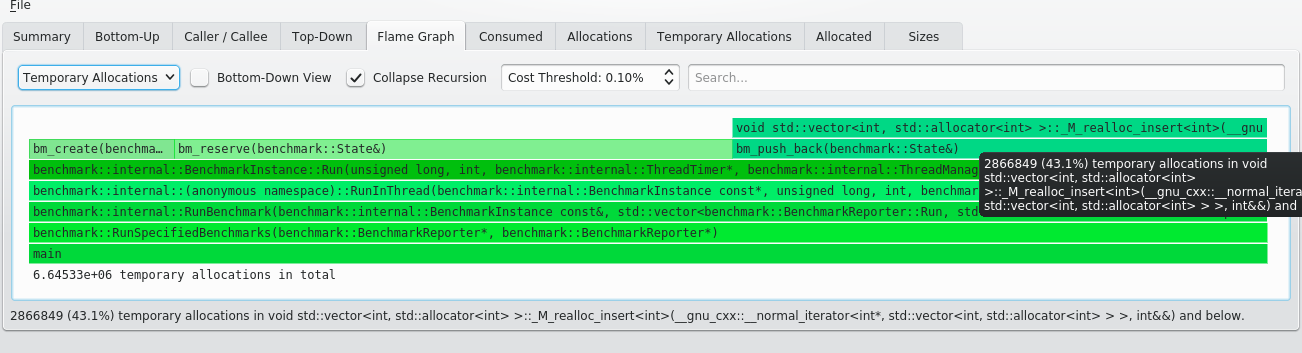
\includegraphics[width=.9\textwidth]{img/heaptrack_gui.png}
	\end{center}
\end{frame}

\subsection{FlameGraph}
\begin{frame}{FlameGraph -- наглядное отображение результатов профилирования}
	\begin{itemize}
		\item Основное:
		\begin{itemize}
			\item снизу вверх располагаются кирпичики-блоки функции в порядке уровня вложенности
			\item блоки вызванных функций располагаются строго на блоках их вызвавших
			\item на одном уровне блоки расположены по ширине соответственно использованию рассматриваемого ресурса
		\end{itemize}
		\item Нужные perl-скрипты располагаются в репозитории \href{https://github.com/brendangregg/FlameGraph}{\beamerbutton{GitHub}}
		\begin{itemize}
			\item stackcollapse-perf.pl -- для работы со срезами стека из perf
			\item flamegraph.pl -- для преобразования полученной из предыдущего скрипта структуры данных интерактивного svg-изображения с искомым флеймграфом.
		\end{itemize}
	\end{itemize}
\end{frame}

\begin{frame}[fragile]{Построение FlameGraph-а}
	\begin{enumerate}
		\item Сохраняем в директорию с результатами профилирования perf.data вышеупомянутые perl-скрипты. Не забываем дать им возможность исполняться, выполнив chmod +x на файлах скриптов.
		\item Получаем срезы стека из perf:
\scriptsize\begin{lstlisting}
   perf script > perf.script 
\end{lstlisting}\normalsize
		\item Обрабатываем первым скриптом:
\scriptsize\begin{lstlisting}
   ./stackcollapse-perf.pl perf.script > perf.folded
\end{lstlisting}\normalsize
		\item Получаем svg-файл вторым скриптом:
\scriptsize\begin{lstlisting}
   ./flamegraph.pl perf.folded > example.svg
\end{lstlisting}\normalsize
	\end{enumerate}
	\vspace{-0.5cm}
	\begin{center}
			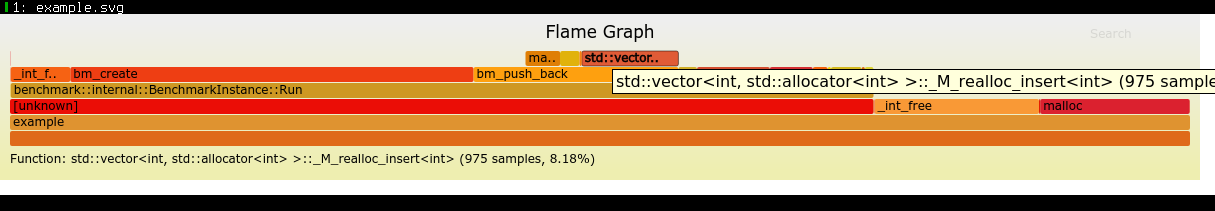
\includegraphics[height=1.8cm]{img/flamegraph.png}
	\end{center}
\end{frame}

